%❖ Chương này tập trung trình bày chi tiết những gì bạn
%làm
%❖ Mô tả chi tiết phương pháp thực hiện, giải pháp đề xuất, ứng dụng phát triển
%❖ Có thể đưa ra ví dụ minh họa để dẫn nhập
%❖ Nên phân thành các mục con
%   
%❖ Hướng nghiên cứu: Phương pháp đề xuất (Proposed Approach)
%o Cơ sở lý thuyết
%o Câu hỏi nghiên cứu, giả thuyết khoa học
%o Phương pháp/Thủ tục thực hiện nghiên cứu (procedure)
%o Đối tượng nghiên cứu
%o Môi trường (phần mềm, thư viện, máy móc, công cụ, v.v...)
%o Mô tả dữ liệu, quá trình thu thập dữ liệu
%o Độ đo để đánh giá (performance metrics)

\chapter{Phương pháp đề xuất}
\label{Chapter3}

%\begin{figure}
%    \centering
%    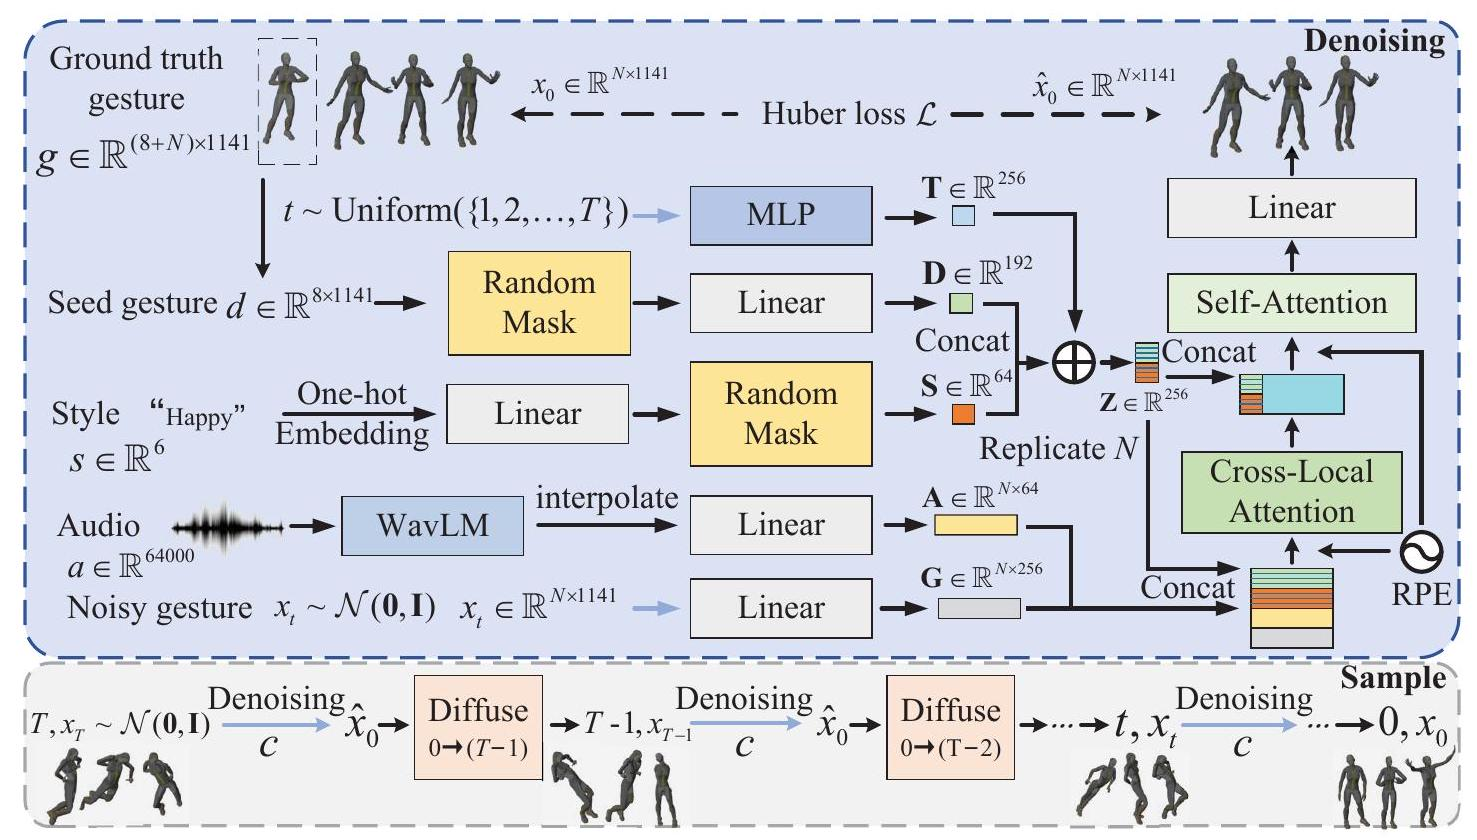
\includegraphics[width=\linewidth]{images/architecture.jpg}
%    \caption{Kiến trúc mồ hình sinh cử chỉ OHGesture}
%    \label{fig:architecture}
%\end{figure}

Bản chất của các phương pháp dựa trên neural network là ước lượng xác xuất của dữ liệu (probability density) nên cần chuẩn hoá (normalization), trong khi mô hình Diffusion sẽ học để có thể ước lượng đạo hàm của phân bố dữ liệu (estimating gradients of data distribution) và không phải chuẩn hoá trên toàn bộ dữ liệu, nên có kết quả tốt hơn so với các phương pháp neuron network không sử dụng diffusion.
Mô hình diffusion có khả năng phủ được phân bố dữ liệu trong các trường hợp mật độ phân bố của dữ liệu thấp  và có thể sinh được kết quả với độ chi tiết cao nên phù hợp với bài toán sinh cử chỉ. Mô hình của chúng tôi dựa trên mô hình DiffuseStyleGesture \cite{yang2022DiffuseStyleGestureplus} với cải tiến để có thể học theo cảm xúc của nhân vật. Trước tiên chúng tôi trình bày về mô hình diffusion \ref{sec:summary_diffusion}, và phần \ref{sec:ohgesture} sẽ trình bày về mô hình đề xuất OHGesture. 

%Diffusion \cite{ho2020denoising} là mô hình được lấy cảm hứng từ mô hình khuếch tán các chất trong hóa học.

\section{Mô hình diffusion cơ bản}
\label{sec:summary_diffusion}

\begin{figure}
	\centering
	\includegraphics[width=\linewidth]{diffusion_forward}
	\caption{Minh hoạ quá trình khử nhiễu (denoising) cử chỉ}
	\label{fig:diffusion_forward}
\end{figure}


Với các phương pháp sử dụng neuron network như ResNet, GAN,.., mục tiêu là tìm được trọng số $\theta$ của hàm $f_{\theta}(x)$, hàm với $x$ là đầu vào, chúng ta sẽ cực tiểu hoá hàm lỗi $\mathcal{L}_\text{loss}$ giữa nhãn $y$ và kết quả dự đoán $\hat{y}$. Sau khi kết thúc quá trình huấn luyện và học được trọng số $\theta'$ ta dự đoán một mẫu dữ liệu mới $x'$ bằng cách forward qua hàm $f_{\theta'}$ để ra được kết quả dự đoán $y'$.

%\begin{figure*}[bp]


Tương tự phương pháp VAE, mã hoá (encode) ma trận đầu vào thành vector tiềm ẩn $z$ và giải mã (decode) vector tiềm ẩn $z$ ngược trở lại ma trận kích thước ban đầu, tuy nhiên mô hình diffusion chia quá trình học thành từng $T$ bước, ở bước thứ $t$ quá trình gây nhiễu (forward diffusion process) $q(\mathbf{x})$ từ $1 \to T$ được thực hiện bằng cách thêm nhiễu $\epsilon \sim \mathcal{N} (\mathbf{0}, \mathbf{I})$ Gaussian (phân phối chuẩn) vào dữ liệu, với trung bình  (mean) bằng $\mathbb{E}[\epsilon]=0$ và độ lệch chuẩn $\operatorname{Var}(\epsilon)=1$, $\mathbf{I}$ là phần tử đơn vị của phân phối chuẩn. Trong hình minh hoạ \ref{fig:diffusion_forward} quá trình giảm nhiễu từ trái qua phải, còn quá trình khử nhiễu từ phải qua trái $p_\theta(x)$. Trong quá trình khử nhiễu (denoising process) từ $T \to 1$, mục tiêu là học được trọng số $\theta$ của hàm dữ đoán nhiễu $f_{\theta}$ hay con được ký hiệu là hàm dự đoán lượng nhiễu ($\epsilon_\theta$) đã được thêm vào. Sau khi kết thúc quá trình học và ta có trọng số $\theta'$ của hàm dự đoán nhiễu $\hat{\epsilon}$ , ta sẽ dùng hàm $f_{\theta'}$ để dự đoán nhiễu. Sau khi có nhiễu dự đoán $\hat{\epsilon}$, ta trừ đi ảnh bị nhiễu $\mathbf{x}_{t}$ để có được ảnh khử nhiễu $\mathbf{x}_{t-1}$, và cộng với nhiễu $ \mathbf{z} \in \mathcal{N}(0, \mathbf{I})$ để tạo ra sự đa dạng cử chỉ. Thực hiện lần lượt từ $T \to 1$ để có được ảnh dự đoán $\hat{x_0}$. Như hình \ref{fig:basic_diffusion} là kiến trúc đầy đủ của mô hình diffusion tiêu chuẩn (Denoising Diffusion Probabilistic Models - DDPM).

\subsection{Quá trình gây nhiễu (forward diffusion process)}

Cho dữ liệu $\mathbf{x}_{0}$ là được lấy từ dữ liệu thật $\mathbf{x}_{0} \sim q(x)$, với mỗi bước ta sẽ thêm nhiễu vào đầu vào $x_{0}$ với tỷ lệ nhiễu và ảnh gốc được kiểm soát bằng hệ số $\beta$:
\vspace{-20pt}
\begin{figure*}
	\centering
	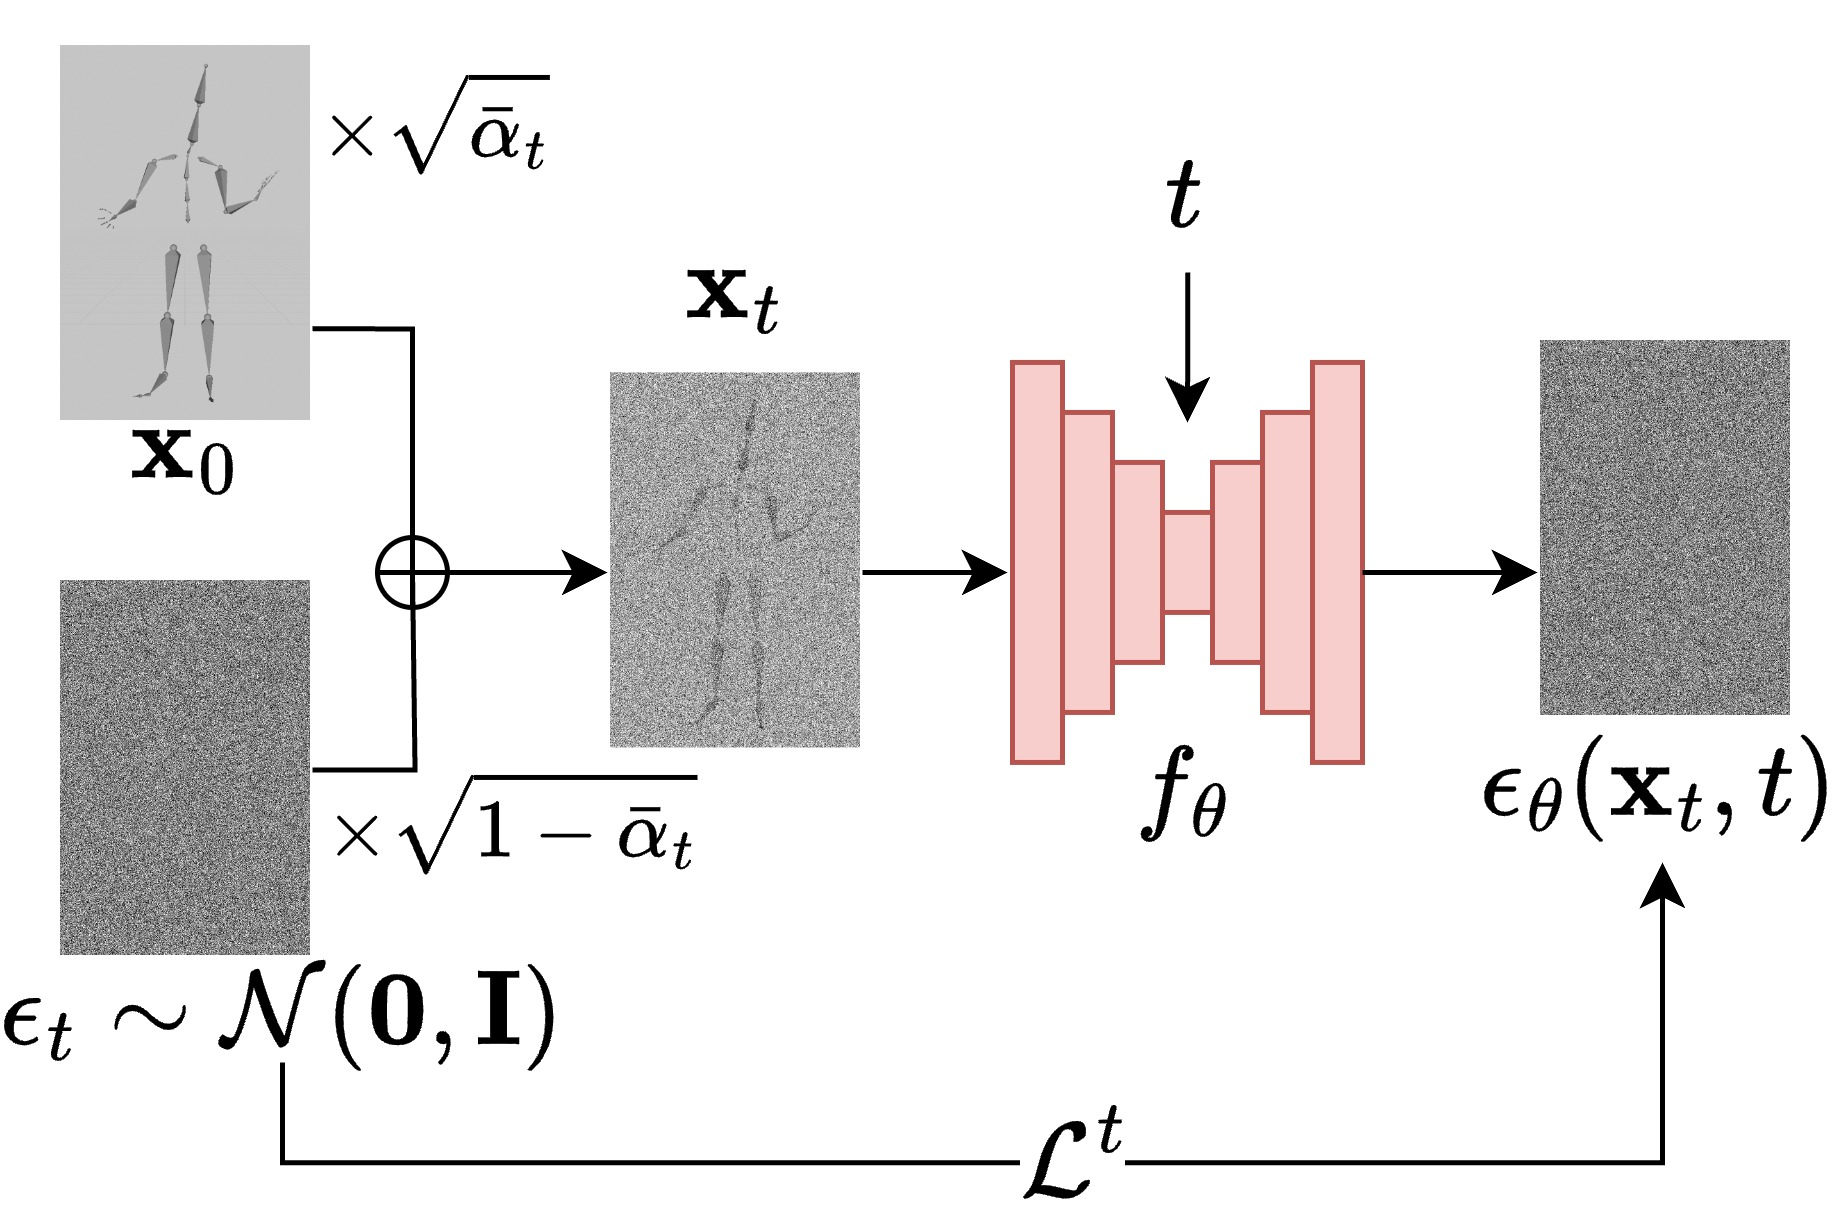
\includegraphics[height=180pt]{AlgorithmForwardDiffusion}
	\vspace{-5pt}
	\caption{Minh hoạ quá trình huấn luyện và làm nhiễu (Diffuse)}
	\label{fig:AlgorithmForwardDiffusion}
	\vspace{-10pt}
\end{figure*}


\begin{equation}
	\label{eq:addgaussian}
	\mathbf{x}_t = \sqrt{1 - \beta_t}\mathbf{x}_{t-1} + \sqrt{\beta_t} \boldsymbol{\epsilon}_{t-1}
\end{equation}

Trong đó, quá trình gây nhiễu từ $1 \to T$, với mỗi bước $t$ quá trình thêm nhiễu $\epsilon$ được điều khiển bằng $\beta_t$ theo phương sai $\{\beta_t \in (0, 1)\}_{t=1}^T$:

\begin{equation}
	\label{eq:forward_diffusion_process}
	\begin{aligned}
		q(\mathbf{x}_t \vert \mathbf{x}_{t-1}) &= \mathcal{N}(\mathbf{x}_t; \sqrt{1 - \beta_t} \mathbf{x}_{t-1}, \beta_t\mathbf{I}) \quad \\
		q(\mathbf{x}_{1:T} \vert \mathbf{x}_0) &= \prod^T_{t=1} q(\mathbf{x}_t \vert \mathbf{x}_{t-1})
	\end{aligned}
\end{equation}

Mục tiêu ở bước $t$ của hệ số $\sqrt{1 - \beta_t}$ và $\beta_t$ là để lần lượt giảm tỷ lệ của ảnh gốc $x_t$ và tăng dần nhiễu  $\boldsymbol{\epsilon}_{t-1}$, vì vậy $\beta_1 < \beta_2 < \dots < \beta_T$. Khi $T \to \infty$ thì $x_{T}$ sẽ hoàn toàn nhiễu (Isotropic Gaussian Distribution) $q(T) = \mathcal{N} (0, \mathbf{I})$.


Vì nhiễu $\boldsymbol{\epsilon}_{t-1}, \boldsymbol{\epsilon}_{t-2}, \dots \sim \mathcal{N}(\mathbf{0}, \mathbf{I})$ luôn luôn là phân phối chuẩn, và cho trước trong mọi bước $t$, nên ta có thể dễ dàng truy ngược được $x_t$ từ $x_0$. Bằng cách đặt $\alpha_t = 1 - \beta_t$ và $\bar{\alpha}_t = \prod_{i=1}^t \alpha_i$, từ công thức \ref{eq:addgaussian}, ta có hàm forward diffusion viết lại theo $\alpha$ như sau:

\begin{equation}
	\label{eq:tracexzero}
	\begin{aligned}
		\mathbf{x}_t 
		&= \sqrt{\alpha_t}\mathbf{x}_{t-1} + \sqrt{1 - \alpha_t}\boldsymbol{\epsilon}_{t-1} \\
		&= \sqrt{\alpha_t \alpha_{t-1}} \mathbf{x}_{t-2} + \sqrt{1 - \alpha_t \alpha_{t-1}} \bar{\boldsymbol{\epsilon}}_{t-2}
		&= \sqrt{\bar{\alpha}_t}\mathbf{x}_0 + \sqrt{1 - \bar{\alpha}_t}\boldsymbol{\epsilon} \\
		q(\mathbf{x}_t \vert \mathbf{x}_0) &= \mathcal{N}(\mathbf{x}_t; \sqrt{\bar{\alpha}_t} \mathbf{x}_0, (1 - \bar{\alpha}_t)\mathbf{I})
	\end{aligned}
\end{equation}


\subsection{Quá trình khử nhiễu (denoising process)}
\label{subsection:denoising_process}

\begin{figure}[]
	\centering
	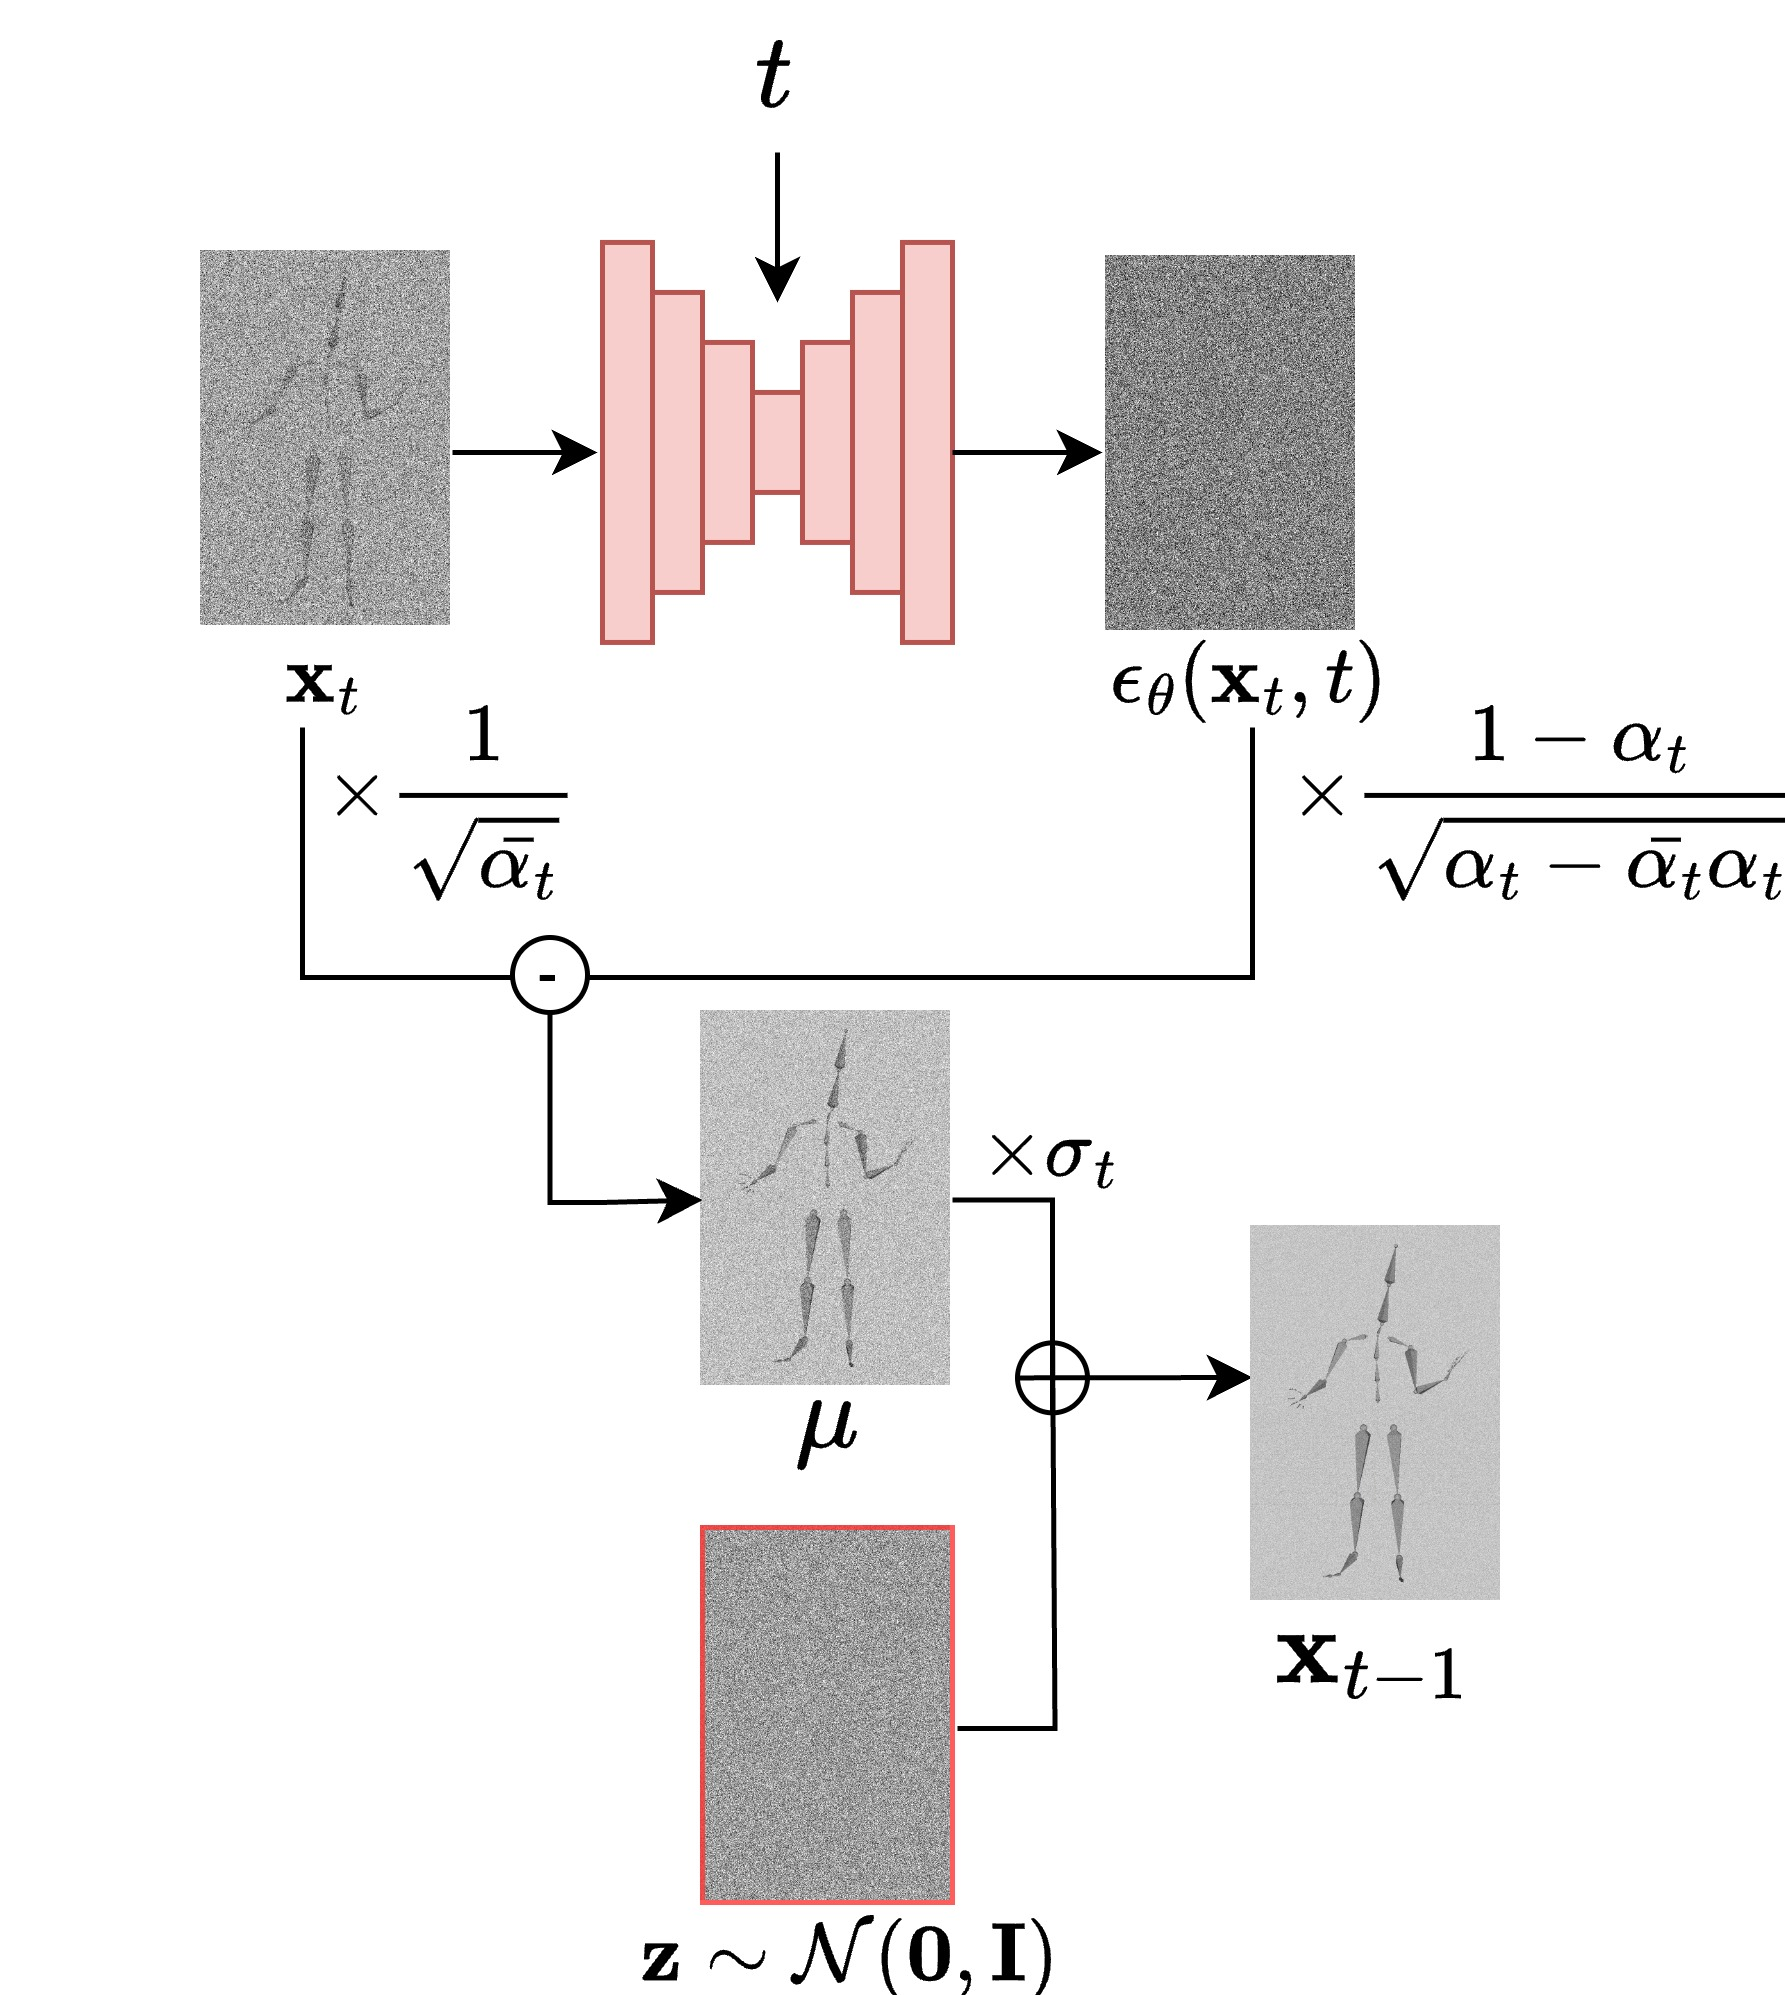
\includegraphics[height=280pt]{AlgorithmSamplingDiffusion.png}
	\caption{Minh hoạ quá trình khử nhiễu (Denoise)}
	\label{fig:AlgorithmSamplingDiffusion}
	\vspace{-20pt}
\end{figure}

Quá trình khử nhiễu $p_\theta(\mathbf{x}_{t-1} \vert \mathbf{x}_t)$  ở bước thứ $t$ từ $T \to 1$ được bắt đầu từ $x_T$ là hoàn toàn nhiễu $\mathcal{N} (\mathbf{0}, \mathbf{I})$. Ta sẽ dùng một neural network $f_{\theta} (x_t, t)$ để dự đoán nhiễu $\hat{\epsilon} = f_{\theta}(x_t, t)$ đã được thêm vào để được $x_{t-1}$ từ $x_t$.

Quá trình khử nhiễu có trung bình $\boldsymbol{\mu}_\theta(\mathbf{x}_t, t) = {\frac{1}{\sqrt{\alpha_t}} \Big( \mathbf{x}_t - \frac{1 - \alpha_t}{\sqrt{1 - \bar{\alpha}_t}}  f_\theta(\mathbf{x}_t, t) \Big)}$ và độ lệch chuẩn $\boldsymbol{\Sigma}_\theta(\mathbf{x}_t, t)$ như sau:


%\begin{equation} \mathrm{d}\mathbf{x} = [\mathbf{f}(\mathbf{x}, t) - g^2(t) \nabla_\mathbf{x} \log p_t(\mathbf{x})]\mathrm{d}t + g(t) \mathrm{d} \mathbf{w}.\label{rsde} \end{equation}

% bằng cách lấy ảnh bị nhiễu trừ đi nhiễu dự đoán

\begin{equation}
	\label{eq:denoising_process}
	\begin{aligned}
		p_\theta(\mathbf{x}_{0:T})
		&= p(\mathbf{x}_T) \prod^T_{t=1} p_\theta(\mathbf{x}_{t-1} \vert \mathbf{x}_t) \\
		p_\theta(\mathbf{x}_{t-1} \vert \mathbf{x}_t) &= \mathcal{N}(\mathbf{x}_{t-1};  \boldsymbol{\mu}_\theta(\mathbf{x}_t, t), \boldsymbol{\Sigma}_\theta(\mathbf{x}_t, t))
	\end{aligned}
\end{equation}

Qúa trình khử nhiễu là quá trình bắt đầu từ nhiễu hoàn toàn, dùng một neuron network $f_\theta$ để học được quá trình khử nhiễu.

%Ta viết lại hàm denoising từ công thức \ref{eq:denoising_process}  theo $\alpha$ như sau:
%$$
%x_{t-1} = \frac{1}{\sqrt{\alpha_t}} \left( x_t - \frac{\sqrt{1 - \alpha_t}}{\sqrt{1 - \bar{\alpha}_t}} \epsilon_{\theta}(x_t, t) \right) + \sqrt{1 - \alpha_t} \tilde{\epsilon}_t
%$$


%\begin{equation}
%	\label{eq:denoising_alpha}
%	\begin{aligned}
	%	p_\theta(\mathbf{x}_{t-1} \vert \mathbf{x}_t) &= \mathcal{N}(\mathbf{x}_{t-1}; \boldsymbol{\mu}_\theta(\mathbf{x}_t, t), \boldsymbol{\Sigma}_\theta(\mathbf{x}_t, t))
	%\end{aligned} \\
	% \bar{\boldsymbol{\mu}}_t (x_t, t) = \frac{1}{\sqrt{\alpha_t}} \Big( \mathbf{x}_t - \frac{1 - \alpha_t}{\sqrt{1 - \bar{\alpha}_t}} \boldsymbol{\epsilon}_t \Big)
	%\end{equation}
	
	\subsection{Quá trình huấn luyện trong mô hình diffusion cơ bản}
%	Hàm mất mát $\mathcal{L}$ của mô hình diffusion
	
	\begin{figure}
		\centering
		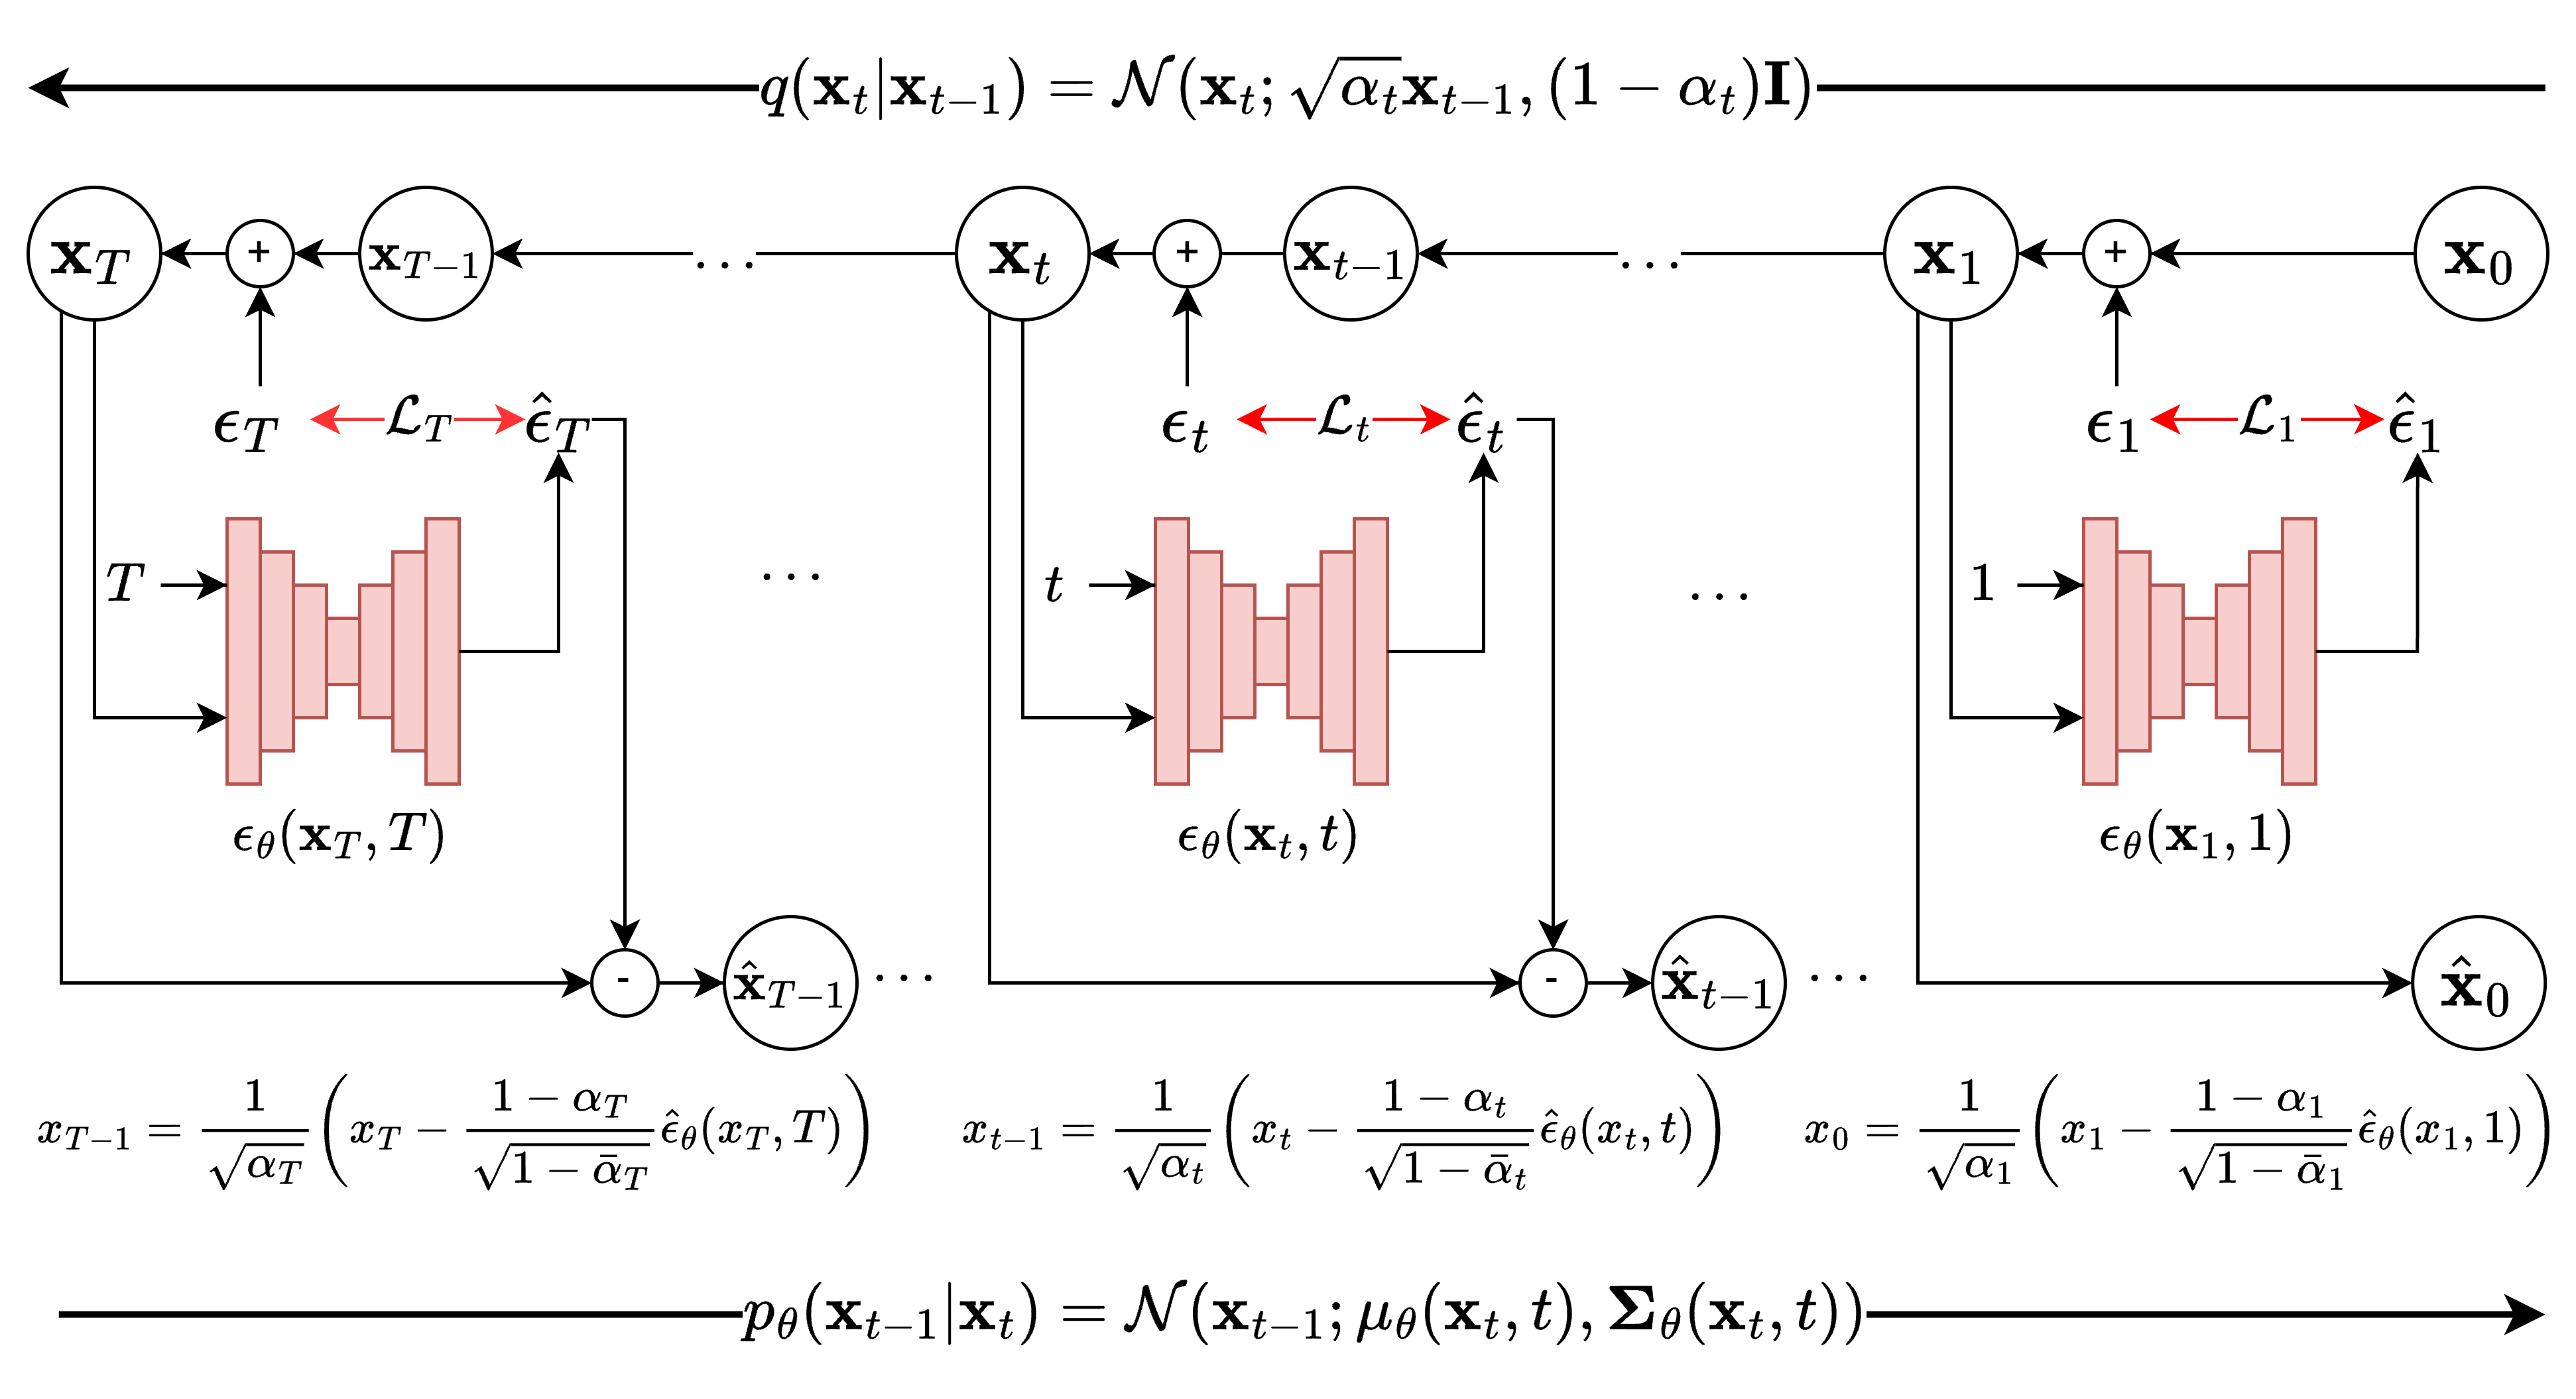
\includegraphics[width=0.8\linewidth]{DDPMTraining}
		\caption{Mô hình diffusion cơ bản}
		\label{fig:basic_diffusion}
	\end{figure}
	
	Mô hình diffusion sẽ học trọng số $\theta$ của hàm dự đoán lỗi $f_{\theta} (x_t, t)$ hay còn ký hiệu là  $\epsilon_{\theta} (x_t, t)$. Trong quá trình denoising, ta sẽ tối ưu độ lỗi giữa nhiễu dự đoán $\boldsymbol{\epsilon}_\theta(\mathbf{x}_t, t)$ và nhiễu thực tế $\boldsymbol{\epsilon}_t$. Với mỗi bước thứ $t$ ta sẽ tối ưu hàm loss $\mathcal{L}_{t}$ để thu được trọng số $\theta$.
	
	\begin{equation}
		\label{eq:diffusion_loss}
		\begin{aligned}
			\mathcal{L}_t
			&= \mathbb{E}_{t \sim [1, T], \mathbf{x}_0, \boldsymbol{\epsilon}_t} \Big[\|\boldsymbol{\epsilon}_t - \boldsymbol{\epsilon}_\theta(\mathbf{x}_t, t)\|^2 \Big] \\
			&= \mathbb{E}_{t \sim [1, T], \mathbf{x}_0, \boldsymbol{\epsilon}_t} \Big[\|\boldsymbol{\epsilon}_t - \boldsymbol{\epsilon}_\theta(\sqrt{\bar{\alpha}_t}\mathbf{x}_0 + \sqrt{1 - \bar{\alpha}_t}\boldsymbol{\epsilon}_t, t)\|^2 \Big]
		\end{aligned}
	\end{equation}
	
	
Với $f_{\theta}(x_{t-1}, t)$ hay $\epsilon_\theta$ là một mô hình Unet dùng để mã hoá và giải mã dữ liệu để dự đoán nhiễu đã thêm vào dữ liệu. Quá trình tính toán hàm lỗi được trình bày minh hoạ trong hình \ref{fig:basic_diffusion}.

\begin{algorithm}
	\caption{Thuật toán training trong DDPM}
	\begin{enumerate}
		\item Tính sẵn các giá trị $\sqrt{\alpha_t}$, $\sqrt{1 - \alpha_t}$ và $\sqrt{\bar{\alpha}_t}$ cho mỗi bước $t: 1 \rightarrow T$. Xác định lịch trình nhiễu $\{\alpha_t \in (0, 1)\}_{t=1}^T$, với $\alpha_1 < \alpha_2 < \dots < \alpha_T$.
		
		\item Lấy nhãn $\mathbf{x}_0$ từ phân phối của dữ liệu đã chuẩn hoá.
		
		\item Tạo nhiễu ngẫu nhiên $\boldsymbol{\epsilon}_t$ cho mỗi bước $t: 1 \rightarrow T$, với $\forall t: \boldsymbol{\epsilon}_t \sim \mathcal{N}(\mathbf{0}, \mathbf{I})$.
		
		\item Gây nhiễu (forward) $\mathbf{x}_0$ để thu được $\mathbf{x}_t$ ở mỗi bước $t: 1 \rightarrow T$:
		$$
		\mathbf{x}_t = \sqrt{\bar{\alpha}_t} \mathbf{x}_0 + \sqrt{1 - \bar{\alpha}_t} \boldsymbol{\epsilon}_t
		$$
		
		\item Với mỗi $t$, lấy $t$ \textbf{ngẫu nhiên} từ $[1, T]$.
		
		\item Cho $\mathbf{x}_t$ và $t$ vào mô hình để dự đoán nhiễu: $\hat{\boldsymbol{\epsilon}} = \boldsymbol{\epsilon}_\theta(\mathbf{x}_t, t)$.
		
		\item Tính đạo hàm để cập nhật trọng số:
		$$
		\grad_{\theta_t} \left\| \boldsymbol{\epsilon}_t - \boldsymbol{\epsilon}_\theta(\mathbf{x}_t, t) \right\|^2
		$$
		Tính loss:
		$$
		\mathcal{L}_t = \mathbb{E}_{t \sim [1, T], \mathbf{x}_0, \boldsymbol{\epsilon}_t} \left[ \|\boldsymbol{\epsilon}_t - \boldsymbol{\epsilon}_\theta(\sqrt{\bar{\alpha}_t} \mathbf{x}_0 + \sqrt{1 - \bar{\alpha}_t} \boldsymbol{\epsilon}_t, t)\|^2 \right]
		$$
		
		\item Quay lại bước 6 cho đến khi hội tụ để thu được trọng số tối ưu $\theta'$.
	\end{enumerate}
\end{algorithm}

%	Lưu ý 
%	Thay vì dùng neuron network để dự đoán phân bố của dữ liệu theo như hình \ref{fig:basic_diffusion}, mô hình diffusion sẽ dự đoán độ lỗi được thêm vào trong ảnh ở bước thứ $t$, với mỗi $t$ bước ta sẽ cần tối ưu hàm mất mát $\mathcal{L}_t$, hàm mất mát của mỗi bước sẽ tối ưu độ lỗi giữa nhiễu dự đoán $\hat{\epsilon_t}$ và nhiễu nhãn $\epsilon_t$ được thêm vào. 
	
	
\subsection{Quá trình lấy mẫu trong diffusion cơ bản}
	
		\begin{figure*}
		\centering
		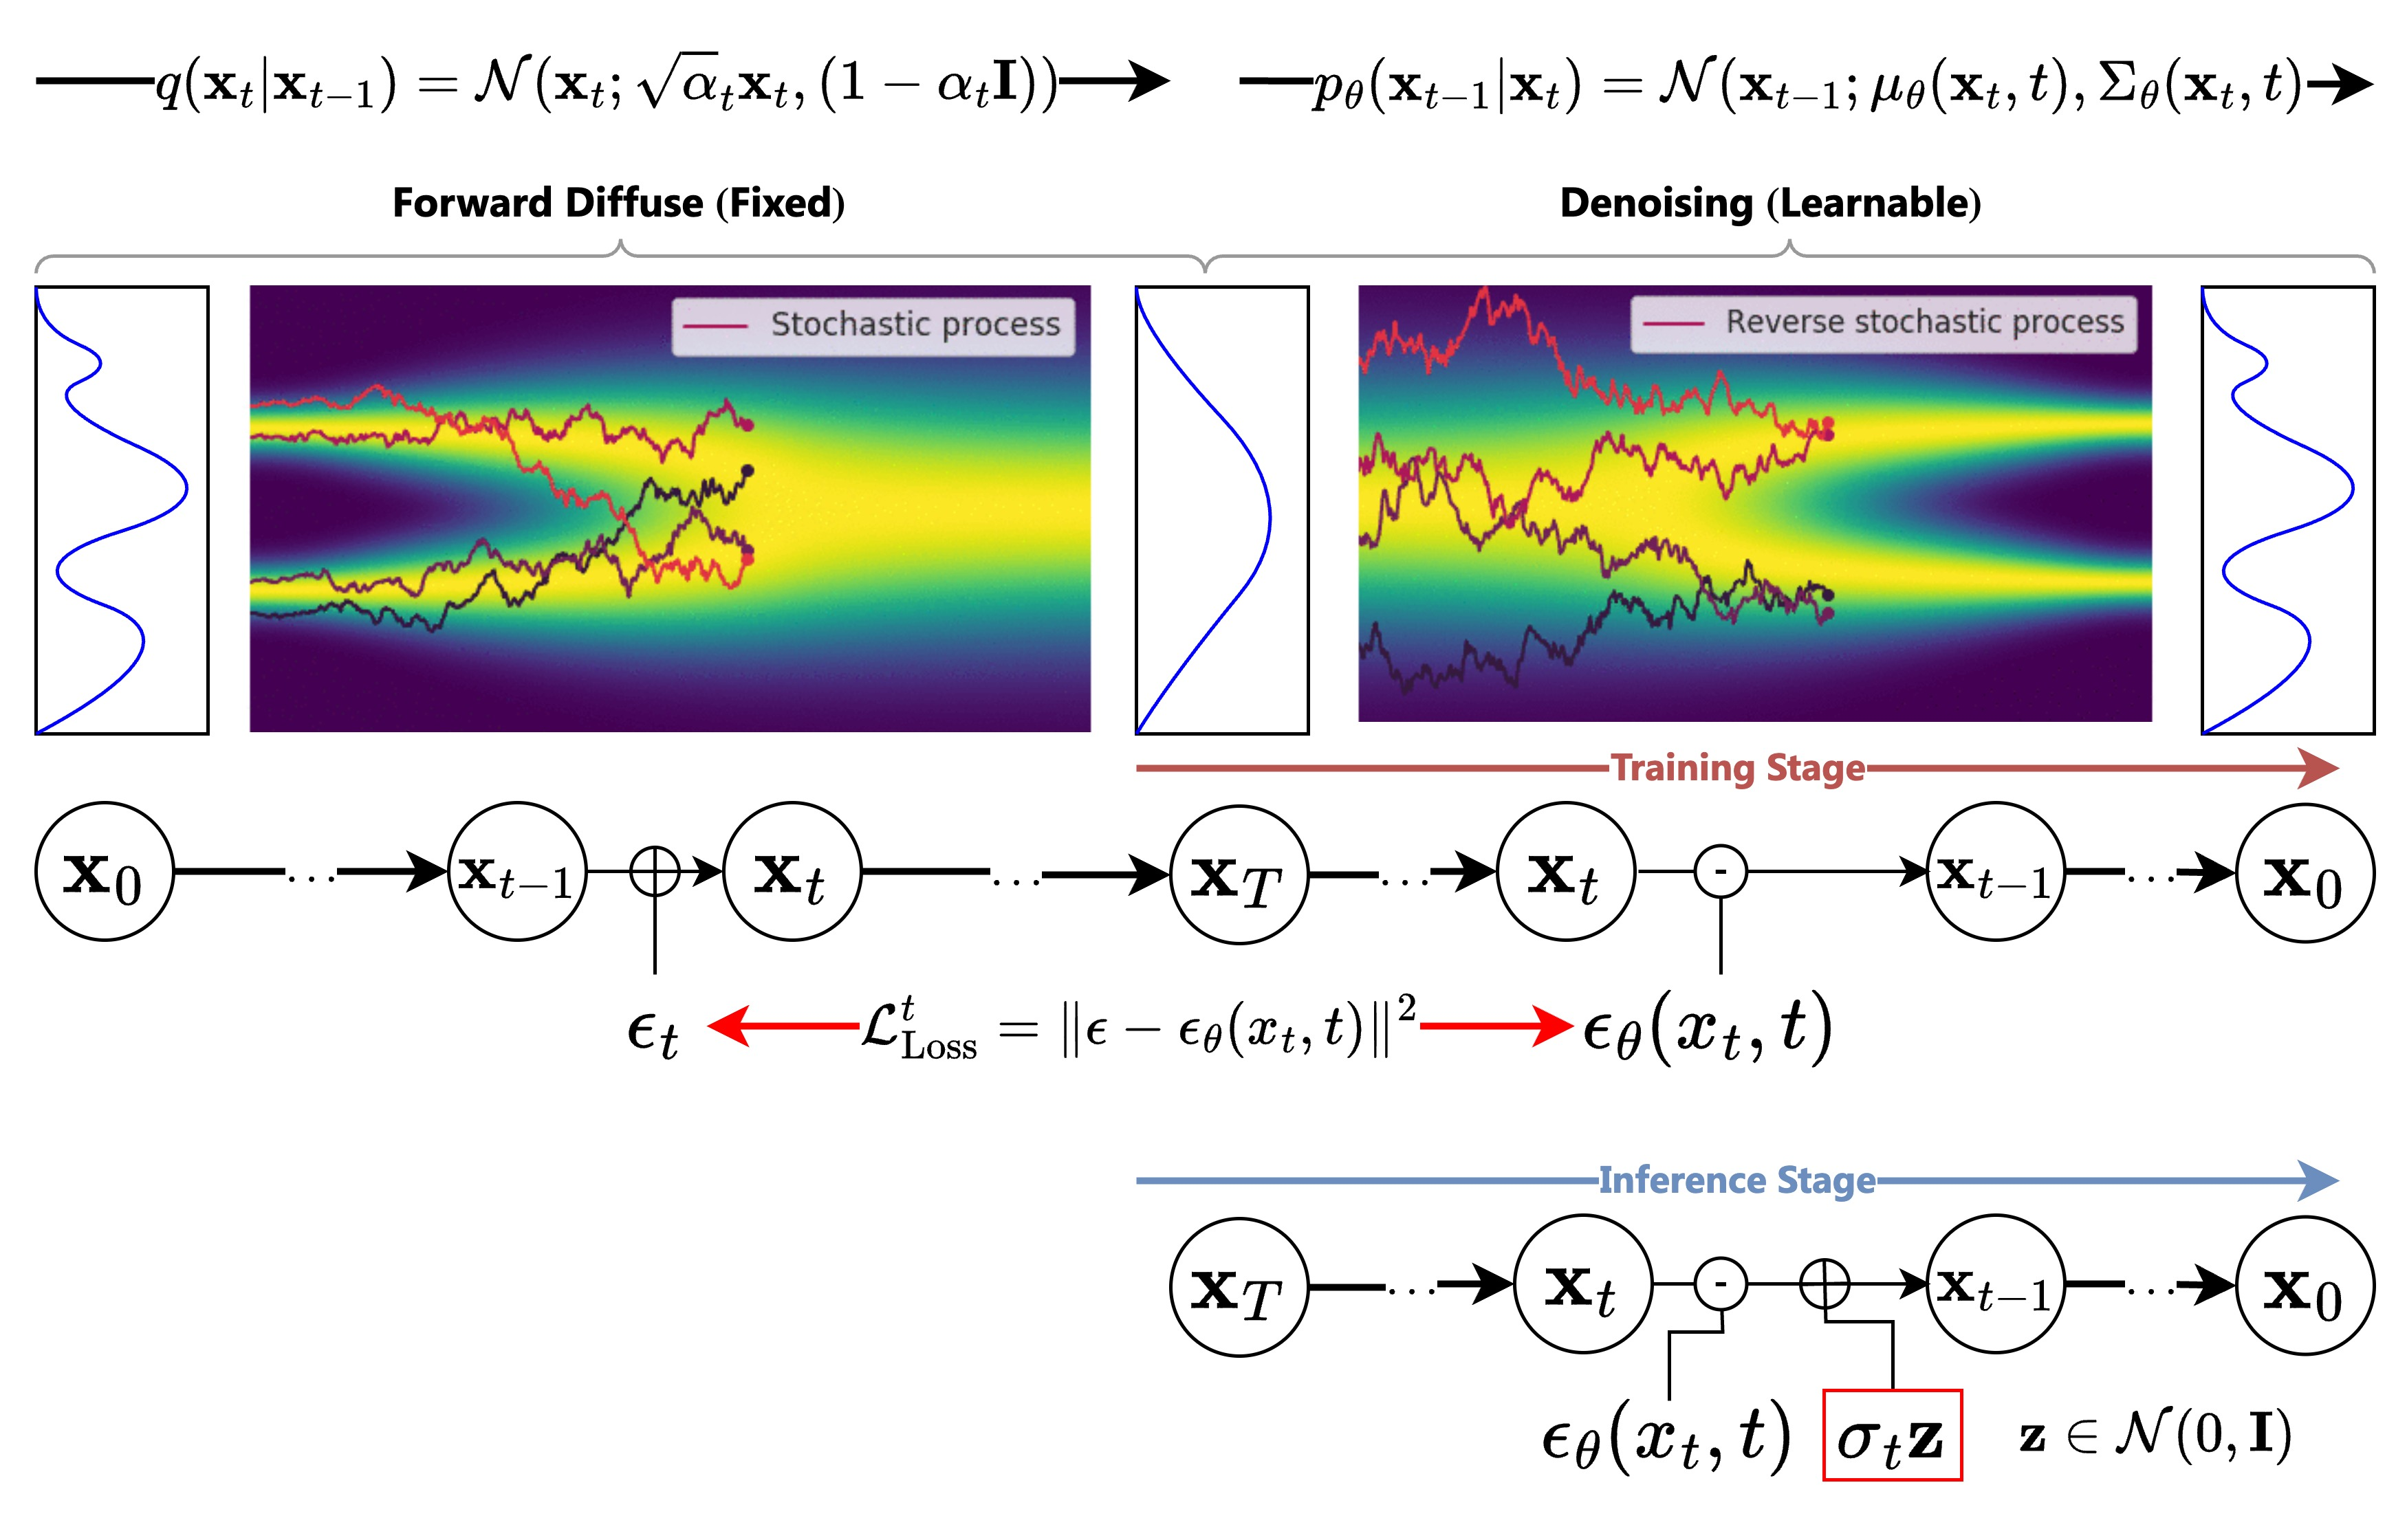
\includegraphics[width=0.8\linewidth]{GaussianDrift}
		\caption{Quá trình Training và Sampling trong mô hình Diffusion tiêu chuẩn}
		\label{fig:GaussianDrift}
	\end{figure*}
	

	Sau khi thu được trọng số $\theta'$, ta sẽ dùng hàm denoising để khử nhiễu từ nhiễu $x_T \sim \mathcal{N} (\mathbf{0}, \mathbf{I})$.
	Quá trình biến đổi từ nhiễu hoàn toàn $x_{T}$ sang dự đoán $\hat{x_0}$ như sau:
	%với $t$ là một vector đã được nhúng vị trí bằng thuật toán nhúng
	
	\begin{equation}
		\label{eq:adddenoising}
		x_{t-1} = \frac{1}{\sqrt{\alpha_t}} \left( x_t - \frac{1- \alpha_t}{\sqrt{1 - \bar{\alpha}_t}} f_{\theta'}(x_t, t) \right) + \sqrt{1 - \alpha_t} \tilde{\epsilon}_t
	\end{equation}
	
Lưu ý rằng $\epsilon_t$ là nhiễu cố định và lấy ngẫu nhiên trước quá trình huấn luyện, chỉ sử dụng lại kết quả ngẫu nhiên trong quá trình forward diffusion \ref{subsection:denoising_process} ở công thức  \ref{eq:addgaussian}. Như hình \ref{fig:GaussianDrift}, độ lỗi $\epsilon_t$ là độ nhiễu của từng bước $t$, và hàm loss  $\mathcal{L}^{t}$ sẽ tính theo từng bước $t$.


Tiếp theo quá trình huấn luyện, thuật toán lấy mẫu (sampling) trong DDPM bắt đầu từ bước tạo nhiễu hoàn toàn, tức là $\mathbf{x}_T \sim \mathcal{N}(0, \mathbf{I})$, nơi dữ liệu ban đầu hoàn toàn là nhiễu. Các giá trị $\sqrt{\alpha_t}$, $\sqrt{1 - \alpha_t}$ và $\sqrt{\bar{\alpha}_t}$, được tính từ quá trình huấn luyện, sẽ được sử dụng trong quá trình lấy mẫu để dự đoán lại dữ liệu gốc $\mathbf{x}_0$. Bước tiếp theo là tính toán hệ số điều chỉnh nhiễu $\sigma_t$, dựa vào lịch trình nhiễu $\alpha_t$ đã xác định trong quá trình huấn luyện. Các giá trị này sẽ ảnh hưởng đến độ nhiễu được thêm vào trong quá trình lấy mẫu ngược.

Thuật toán lấy mẫu sẽ được thực hiện từ bước $T$ trở về $1$, và trong mỗi bước, một nhiễu ngẫu nhiên $\mathbf{z} \sim \mathcal{N}(0, \mathbf{I})$ được tạo ra để cộng thêm vào kết quả dự đoán. Tại mỗi bước $t$, mô hình sẽ dự đoán nhiễu $\boldsymbol{\epsilon}_{\theta'}$ dựa trên dữ liệu nhiễu $\mathbf{x}_t$ và bước thời gian $t$, sau đó sử dụng dự đoán này để tính toán giá trị $\mu$, là ước lượng của $\mathbf{x}_0$. Cuối cùng, một lượng nhiễu $\sigma_t \mathbf{z}$ được cộng thêm vào $\mu$ để thu được $\hat{\mathbf{x}}{t-1}$, dữ liệu nhiễu tại bước $t-1$. Quá trình này tiếp tục cho đến khi $t = 1$, và khi đó, chúng ta có được $\hat{\mathbf{x}}_0$ — dự đoán cuối cùng của dữ liệu gốc từ quá trình khử nhiễu.

%Mục tiêu của quá trình lấy mẫu này là phục hồi lại dữ liệu ban đầu $\mathbf{x}_0$ từ nhiễu hoàn toàn, đồng thời đảm bảo tính ổn định và sự đa dạng trong quá trình sinh mẫu thông qua việc sử dụng nhiễu ngẫu nhiên $\mathbf{z}$.


\begin{algorithm}
	\caption{Thuật toán sampling trong DDPM}
	\begin{enumerate}
		\item Bắt đầu với nhiễu: $\mathbf{x}_T \sim \mathcal{N}(0, \mathbf{I})$.
		
		\item Các giá trị $\sqrt{\alpha_t}$, $\sqrt{1 - \alpha_t}$ và $\sqrt{\bar{\alpha}_t}$ được lấy từ quá trình huấn luyện.
		
		\item Tính hệ số điều chỉnh nhiễu $\sigma_t$ từ $\alpha_t$ ở mỗi bước $t: 1 \rightarrow T$:
		\[
		\sigma_t = \sqrt{\frac{1 - \bar{\alpha}_{t-1}}{1 - \bar{\alpha}_t} (1 - \alpha_t)}
		\]
		
		\item Với mỗi $t$, lấy $t$ \textbf{tuần tự} từ $[T, \dots, 1]$.
		
		\item Tạo nhiễu ngẫu nhiên $\mathbf{z} \sim \mathcal{N}(0, \mathbf{I})$.
		
		\item Đưa $\mathbf{x}_t$ vào mô hình để suy luận nhiễu: $\boldsymbol{\epsilon}_{\theta'} = \boldsymbol{\epsilon}_{\theta'}(\mathbf{x}_t, t)$.
		
		\item Dùng nhiễu dự đoán để trừ đi $\mathbf{x}_t$ ở bước $t$:
		\[
		\mu = \frac{1}{\sqrt{\alpha_t}} \left( \mathbf{x}_t - \frac{1 - \alpha_t}{\sqrt{1 - \bar{\alpha}_t}} \boldsymbol{\epsilon}_{\theta'}(\mathbf{x}_t, t) \right)
		\]
		
		\item Cộng thêm một lượng nhiễu: $\hat{\mathbf{x}}_{t-1} = \mu + \sigma_t \mathbf{z}$.
		
		\item Khi $t = 1$, thu được $\hat{\mathbf{x}}_0$ từ quá trình khử nhiễu.
	\end{enumerate}
	\label{alg:samplingddpm}
\end{algorithm}

Điều quan trọng nhất trong quá trình lấy mẫu (denoising sampling) đó chính là phải cộng thêm một độ nhiễu $\mathbf{z} \in \mathcal{N}(0, \mathbf{I})$, với $\mathbf{z}$  sẽ được lần lượt thêm ở từng bước $t$ bằng hệ số điều khiển $\sigma_t$. Mục tiêu của nhiễu $\epsilon$ là để  làm gờ phân phối (marginal noise distribution) cho mô hình $f_\theta$ (hay $\epsilon_{\theta}$) có thể học được nhiễu, còn với  $\mathbf{z}$ là để tăng tính đa dạng trong quá trình sinh và sự ổn định trong quá trình lấy mẫu. Thuật toán lấy mẫu được trình bày ở \ref{alg:samplingddpm}


